\documentclass[a4paper,11pt]{article}
%%%%%%%%%%%%%%%%%%%%%%%%%%%%%%%%%%%%%%%%%%%%%%%%%%%%%%%%%%%%%%%%%%%%%%%%%%%%%%%%%%%%%%%%%%%%%%%%%%%%%%%%%%%%%%%%%%%%%%%%%%%%
\usepackage[T1]{fontenc}
\usepackage[utf8]{inputenc}
\usepackage[dvipdfm]{graphicx}
\usepackage{graphics,latexsym}
\usepackage{amsmath}
%%\usepackage[sort,comma,authoryear,round]{natbib}
\usepackage[dvips]{color}
\usepackage{subfigure}
\usepackage{verbatim}
\usepackage[spanish]{babel}
\usepackage[utf8]{inputenc}
\usepackage{graphicx}
\usepackage{subfigure}
\usepackage{appendix}
\usepackage[style=authoryear,citestyle=authoryear,natbib=true,backend=bibtex]{biblatex}

\addbibresource{biblio1.bib}
\setlength\bibitemsep{1.5\itemsep}

\graphicspath{{./figuras/}}

%%\bibpunct{(}{)}{;}{a}{,}{,}

\textheight 24cm \textwidth 17cm \topmargin-2cm
%% \evensidemargin   -0.25cm
\oddsidemargin-0.2cm
%\pagestyle{empty}
\renewcommand{\baselinestretch}{1}

\graphicspath{{./figuras/}}

\begin{document}


\title{Memorias basadas en ADN}


\author{{Andr\'es Herranz Gonz\'alez}\\
{\small Departamento de Inteligencia Artificial, Universidad Polit\'ecnica de Madrid, Spain}}

\date{}
\maketitle

%\title{}

%\address{}

\begin{abstract}

A medida que la información digital continúa aumentando, se necesitan soluciones de almacenamiento de mayor densidad y a más largo plazo. El ADN tiene muchas ventajas potenciales como medio para el almacenamiento de información. Por ejemplo, el ADN tiene una capacidad teórica de almacenamiento de hasta 1 exabyte por milímetro cúbico de ADN, número muy superior a las capacidades alcanzadas con otros métodos tradicionales. Además, las nuevas técnicas de codificación permiten leer los datos incluso habiendo sufrido daños en alguna parte de la memoria, y las células pueden llegar a vivir hasta 500 años. Todas estas ventajas y la gran cantidad de estudios recientes señalan al ADN con una fuente potencial de computación y una opción viable para el almacenamiento masivo de información.

\end{abstract}


\ \\
\textbf{\textit{Keywords}}: ADN; memorias biológicas; almacenamiento; biología programable


\section{Introducción}

Con el empleo de sistemas digitales para la generación, transmisión y almacenamiento de información, surge la necesidad de un mantenimiento activo y continuo de los medios digitales. Las enormes cantidades de datos con las que se trabaja hoy en día generan el problema de disponer de suficiente espacio de almacenamiento. Esta demanda está aumentando rápidamente día a día. El almacenamiento total de información de todo el mundo fue de alrededor de 2.7 ZB en 2012 y cada año, este valor aumenta entorno a un 50\% \citep{Hakami2015}.

La mayoría de los datos del mundo hoy en día se almacenan en medios magnéticos y ópticos \citep{IDC}. Estas tecnologías han mejorado en los últimos años y se han llegado a conseguir capacidades de 185 TB \citep{Sony} con una densidad de aproximadamente 10 GB / mm3. Otras investigaciones recientes demuestran la viabilidad de almacenar 1 PB \citep{ExtremeTech} en discos ópticos, lo que significa una densidad de aproximadamente 100 GB / mm3. A pesar de estas mejoras, el almacenamiento de zettabytes de datos aún necesitaría millones de unidades y usaría un espacio físico significativo. 

La durabilidad de las memorias es otro aspecto importante a tener en cuenta. Los discos ópticos tienen una vida util de entre 3 y 5 años, y las cintas magnéticas entre 10 y 30 años. Las soluciones actuales de almacenamiento de archivos a largo plazo requieren un mantenimiento para limpiar datos corruptos y reemplazar unidades defectuosas. Si se quieren preservar los datos, se debe encontrar una nueva propuesta para el almacenamiento con una mayor densidad y durabilidad.

Las secuencias de ADN sintético se han considerado como un medio potencial para el almacenamiento de datos digitales. El ADN es una opción atractiva porque es muy denso, con un límite teórico superior a 1 EB / mm3 (ocho órdenes de magnitud más denso que las cintas magnéticas) y de larga duración, con una vida media observada de más de 500 años \citep{Allentoft2012}. Además, dada la gran expectación que está teniendo la computación con ADN, es una tecnología con un potencial enorme y un gran soporte de la comunidad investigadora. 

El proceso que conforma el almacenamiento de información en memorias de ADN es: mapeo de los datos digitales en secuencias de nucleótidos de ADN (un nucleótido es el componente básico del ADN), síntesis (fabricación) de las moléculas de ADN correspondientes y finalmente su almacenaje. Por otro lado, la lectura de los datos implica la secuenciación de las moléculas de ADN y la decodificación de la información para obtener los datos originales. 

En las últimas décadas, la computación con ADN y el almacenamiento de información en células ha mejorado exponencialmente. Algunos trabajos de finales de 1990 tales como Microvenus \citep{JoeDavis1996}  y Génesis \citep{EK1999} (que se comentarán  en la Sección 2.4), sentaron las bases de la tecnología e iniciaron una amplia investigación en el campo. Todo ello ha dado lugar a proyectos y técnicas innovadoras \citep{Goldman2013} \citep{Quadri2004} que han facilitado la expansión y mejora de este tipo de memorias. Además, la gran reducción en el coste de síntesis de ADN en los últimos años ha favorecido enormemente el desarrollo de este tipo de proyectos.

\subsection{PCR: Polymerase chain reaction}

La reacción en cadena de la polimerasa (PCR) es un método ampliamente utilizado en biología molecular para hacer un gran número de copias de un segmento de ADN específico. Usando la PCR, una sola copia (o más) de una secuencia de ADN es amplificada exponencialmente.

La gran mayoría de los métodos de PCR se basan en ciclos térmicos. Los ciclos térmicos exponen los reactivos a ciclos repetidos de calentamiento y enfriamiento para permitir que se produzcan diferentes reacciones dependientes de la temperatura, específicamente la fusión del ADN y la replicación del ADN impulsada por enzimas. La PCR emplea dos reactivos principales: cebadores (fragmentos cortos de ADN de una sola cadena conocidos como oligonucleótidos, que son una secuencia complementaria de la de la cabecera del ADN objetivo) y un ADN polimerasa. En el primer paso de la PCR, las dos cadenas de la doble hélice del ADN se separan físicamente a una temperatura elevada en un proceso llamado fusión del ADN. En el segundo paso, la temperatura se reduce y los cebadores se unen a las secuencias complementarias del ADN. Las dos cadenas de ADN se convierten en plantillas para que la ADN polimerasa genere una nueva cadena de ADN a partir de nucleótidos libres. A medida que avanza la PCR, el ADN generado se utiliza como plantilla para la replicación, poniendo en marcha una reacción en cadena en la que la plantilla de ADN original se amplifica exponencialmente.


\section{Estado del arte} 

En esta sección se van a describir y comentar brevemente algunas de las técnicas utilizadas a lo largo de los últimos años para codificar la información y almacenarla posteriormente en cadenas de ADN. Además, se hará un recorrido cronológico de los mayores descubrimientos en los últimos años y los hitos más relevantes en este campo.

Las técnicas recogidas en este apartado no son todas las que hay en la literatura, pero sí son las más reconocidas y las que utilizan como referente otros autores para comparar sus nuevas propuestas. 

Estas técnicas han ido evolucionando y perfeccionándose a lo largo de los años a fin de mejorar la robustez y fiabilidad de los sistemas basados en ADN, ya que generalmente se producen algunos errores en la transcripción o secuenciación de los datos.

\subsection{Representación de los datos}

Las representaciones de los datos a las que estamos acostumbrados (\textit{ASCII, UTF-8}…) no se pueden introducir directamente en el ADN ya que solo disponemos de cuatro nucleótidos diferentes (\textit{A, C, G} y \textit{T}). Por ello, a lo largo del tiempo se han propuesto diversas estrategias para tratar la información y representarla en una estructura cuaternaria (de base 4).

El enfoque más sencillo e intuitivo para almacenar datos binarios en el ADN es trasladar los datos binarios a base 4, generando una cadena de \textit{n / 2} dígitos cuaternarios a partir de una cadena de \textit{n} bits binarios. Los dígitos cuaternarios se pueden asignar a los nucleótidos de ADN (por ejemplo, mapeando \textit{0, 1, 2, 3} -a- \textit{A, C, G, T}, respectivamente). De esta manera, la cadena binaria \textit{01110001} se transformaría en la cadena base 4 siguiente: \textit{1301}, y luego en la secuencia de ADN \textit{CTAC}. Sin embargo, los procesos de síntesis y secuenciación de ADN son propensos a una gran variedad de errores (sustituciones, inserciones y eliminaciones de nucleótidos), lo que requiere una codificación más cuidadosa y robusta.

\subsubsection{Método Huffman}

La probabilidad de algunos de los errores antes mencionados puede reducirse mediante la codificación de datos binarios en base 3 en lugar de base 4 \citep{Goldman2013}, como se ilustra en la Figura \ref{fig:huffman1} (a). El código ternario se transforma en nucleótidos de ADN utilizando un sistema recursivo (Figura \ref{fig:huffman1} (b)) que evita repetir el mismo nucleótido dos veces consecutivas. Esta codificación evita los \textit{homopolimeros}- repeticiones del mismo nucleótido que aumentan significativamente la probabilidad de errores de secuenciación \citep{Niedringhaus2011}.

\begin{figure}[h!]
\begin{center}
 \subfigure[Conversión de binario a nucleótidos de ADN con la codificación Huffman]{
 	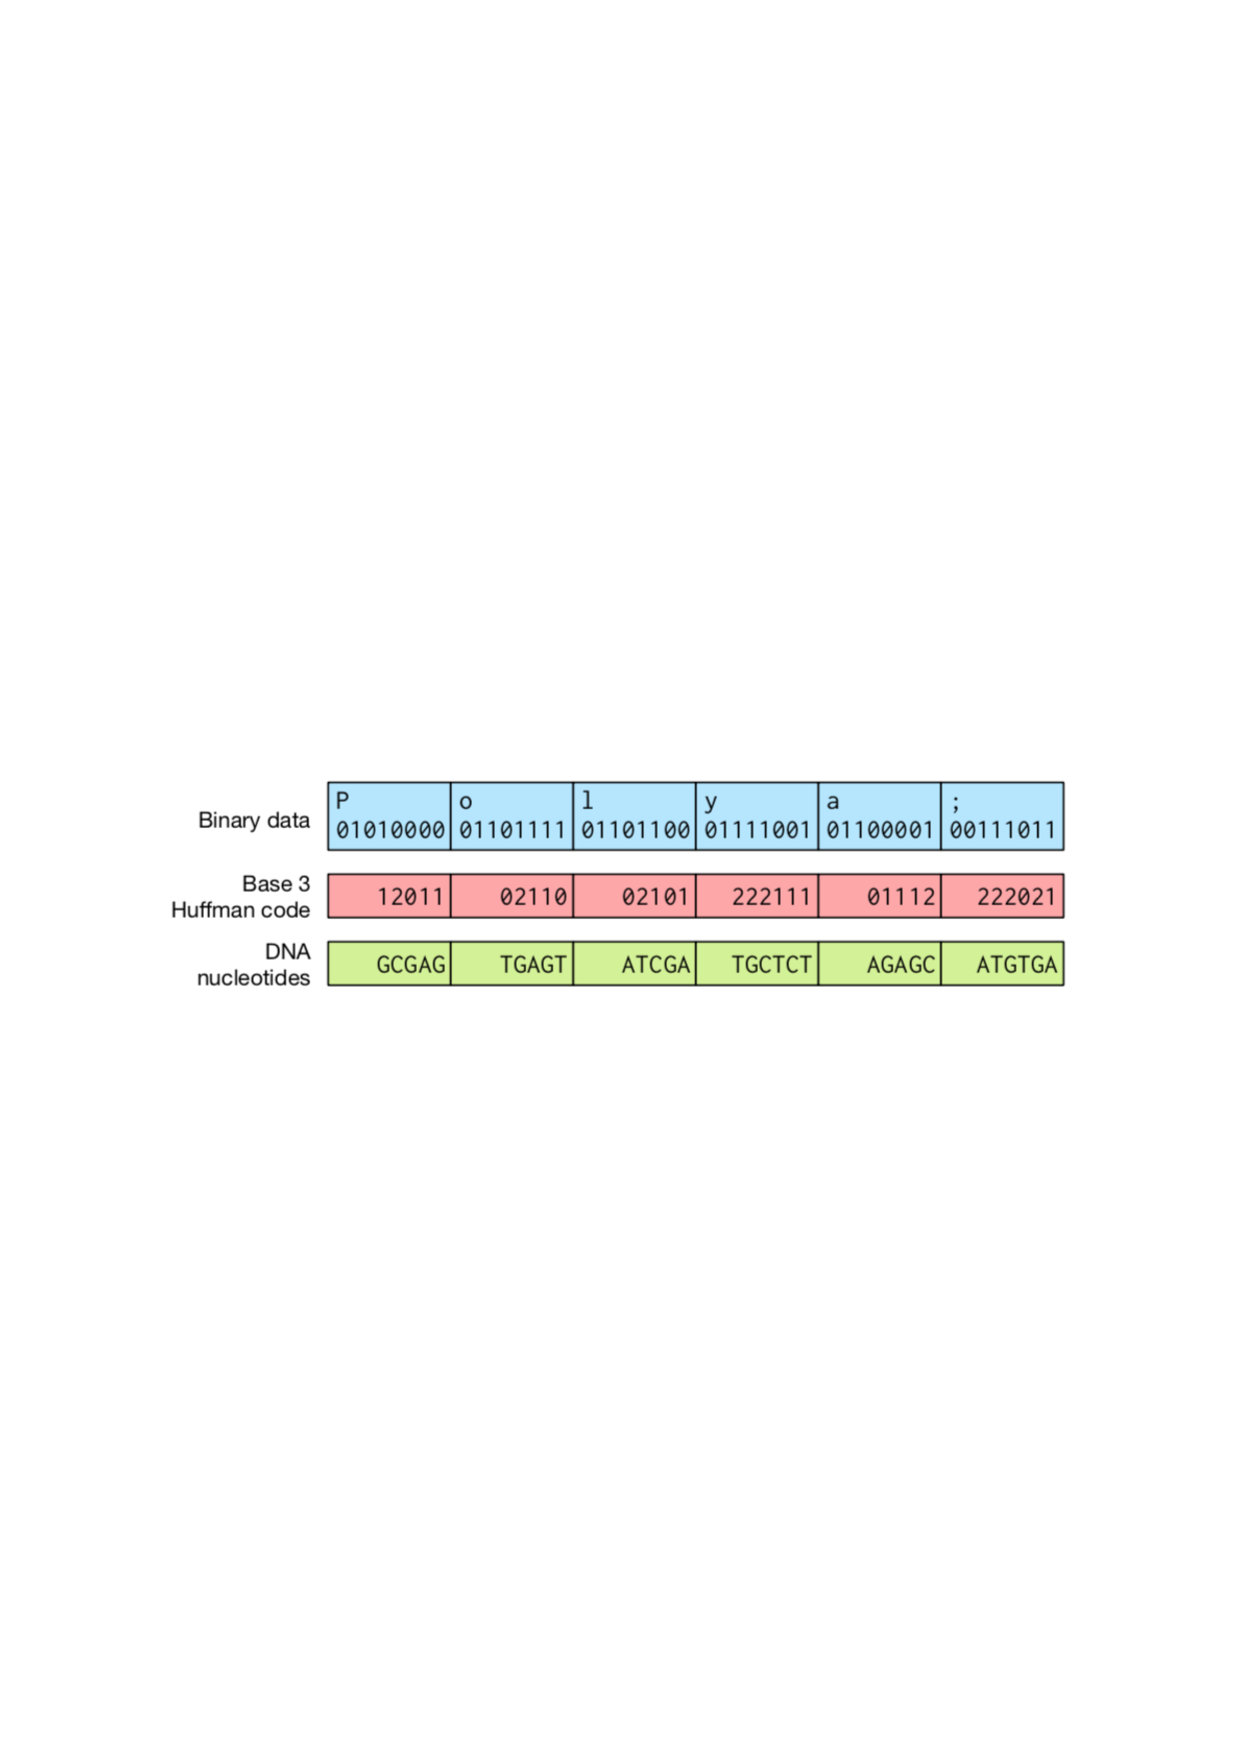
\includegraphics[width=10cm]{huffman-1.pdf}
 }
 \subfigure[Sistema de rotación recursivo para evitar \textit{homopolimeros}]{
 	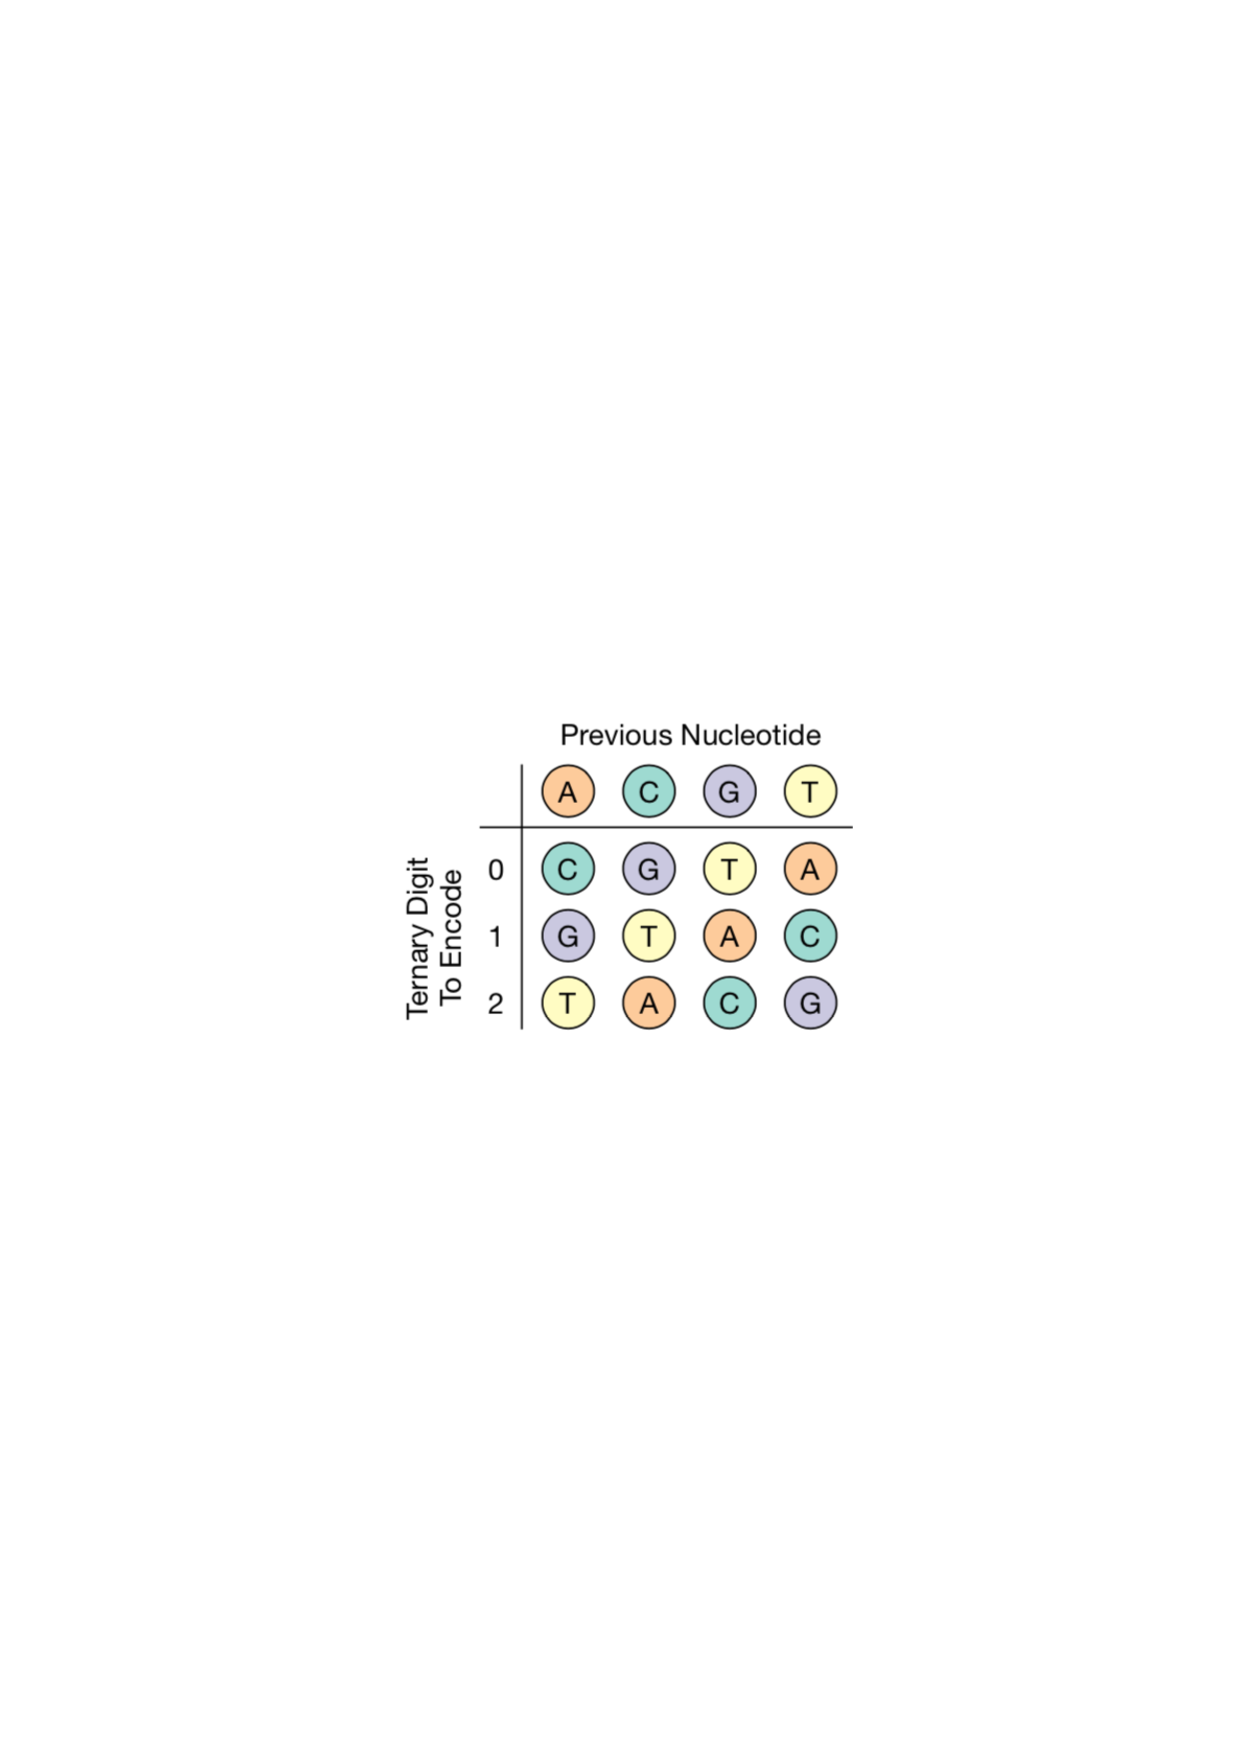
\includegraphics[width=5cm]{huffman-2.pdf}
 }
 \caption{Codificación Huffman}
 \label{fig:huffman1}
 \end{center}
\end{figure}

Debido a que la base 3 no es un múltiplo de la base 2, el mapeo directo entre las bases sería ineficaz: 6 dígitos ternarios ($3^{6}$ = 792) se pueden almacenar 9 bits de datos ($2^{9}$ = 512), pero desperdiciar 217 estados posibles. En su lugar, se propuso la codificación de \cite{HUFFMANt1952} que asigna cada byte binario a 5 o 6 dígitos ternarios. Esto se debe a que 8 dígitos binarios ($2^{8}$ = 256) no se pueden almacenar en 5 dígitos ternarios ($3^{5}$ = 243), ya que nos faltarían 13 valores por representar. Por este motivo, la última posición de la Figura \ref{fig:huffman1} (a) tiene un dígito más y corresponde a uno de estos 13 valores binarios \textit{00111011} que se representa con 6 dígitos ternarios: \textit{222021}. Así, la secuencia de nucleótidos asignado a esta cadena con el sistema recursivo previamente comentado sería: \textit{ATGTGA}.

\subsubsection{Método de reescritura}

Uno de los grandes desafíos de las memorias basadas en ADN es la sobreescritura, es decir, poder actualizar o modificar los datos almacenados sin tener que borrar todas las cadenas de ADN y sin tener que extraer el contenido de todas ellas para después reescribirlo en otras nuevas.

Recientemente, \citep{Chandrasekaran2017} propusieron una nueva técnica de representación de bits basada en \textit{hairpins}. El objetivo de la investigación era demostrar que se podía codificar una memoria de n bits, generando para cada bit un tamaño del \textit{loop} diferente. Tal y como se puede ver en la Figura \ref{fig:reescritura1}, en función del bit que queramos representar, se utiliza un \textit{oligo} que sea complementario a las posiciones que se quieran unir y en función de la distancia entre los \textit{toeholds}, se obtendrá un \textit{hairpins}más grande o más pequeño.

\begin{figure}[h!]
\begin{center}
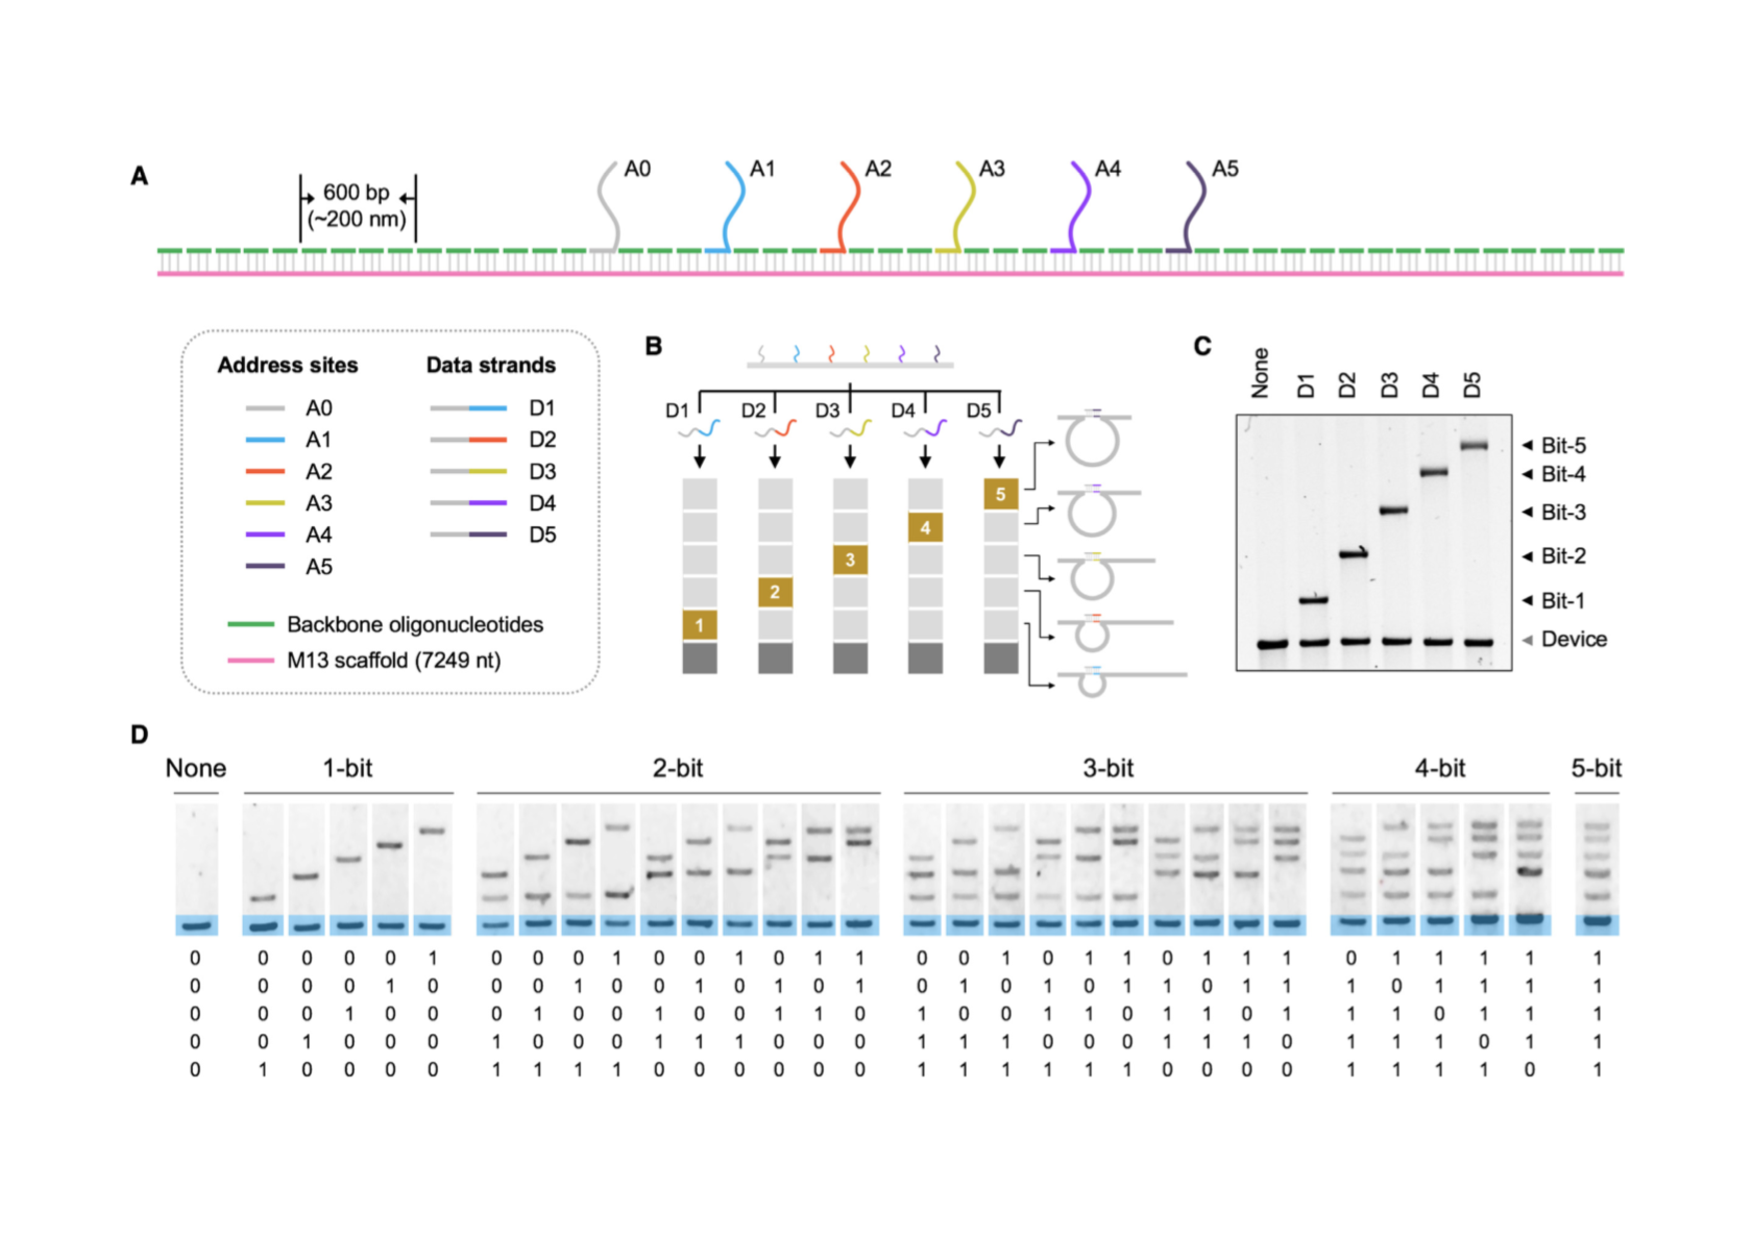
\includegraphics[width=0.85\linewidth]{reescritura-1.pdf}
\caption{Diseño y funcionamiento del sistema de memoria. (A) Diseño del sistema de memoria de 5 bits con múltiples direcciones (A0-A5) que son en parte complementarios a las cadenas de datos (D1-D5). La unión de diferentes cadenas de datos en las posiciones de direccionamiento produce \textit{ hairpins} de diferentes tamaños. (B) Esquema que muestra el funcionamiento del sistema de memoria produciendo diferentes salidas (bits) para diferentes cadenas de datos. Por ejemplo, la cadena gris y azul D1 se unen a las posiciones de direcciones A0 (gris) y A1 (azul) respectivamente, formando así un bucle. (C) Lectura en gel del sistema de memoria de 5 bits. (D) Lectura en gel de todas las combinaciones de bits posibles utilizando el sistema de memoria de 5 bits.}
\label{fig:reescritura1}
\end{center}
\end{figure}

Además, este tipo de representación y codificación permite la reescritura tal y como se muestra en la Figura \ref{fig:reescritura2}. Esto es posible si al utilizar el \textit{oligo} complementario de los dos \textit{toeholds} que queremos unir, añadimos un segmento que quede libre en la unión. De esta manera, si más adelante se quieren modificar los datos, sencillamente habría que deshacer el \textit{hairpins} utilizando el complementario del segmento que había quedado suelto, y utilizar de nuevo otra cadena generar el nuevo bit (\textit{loop}) que queremos representar.

\begin{figure}[h!]
\begin{center}
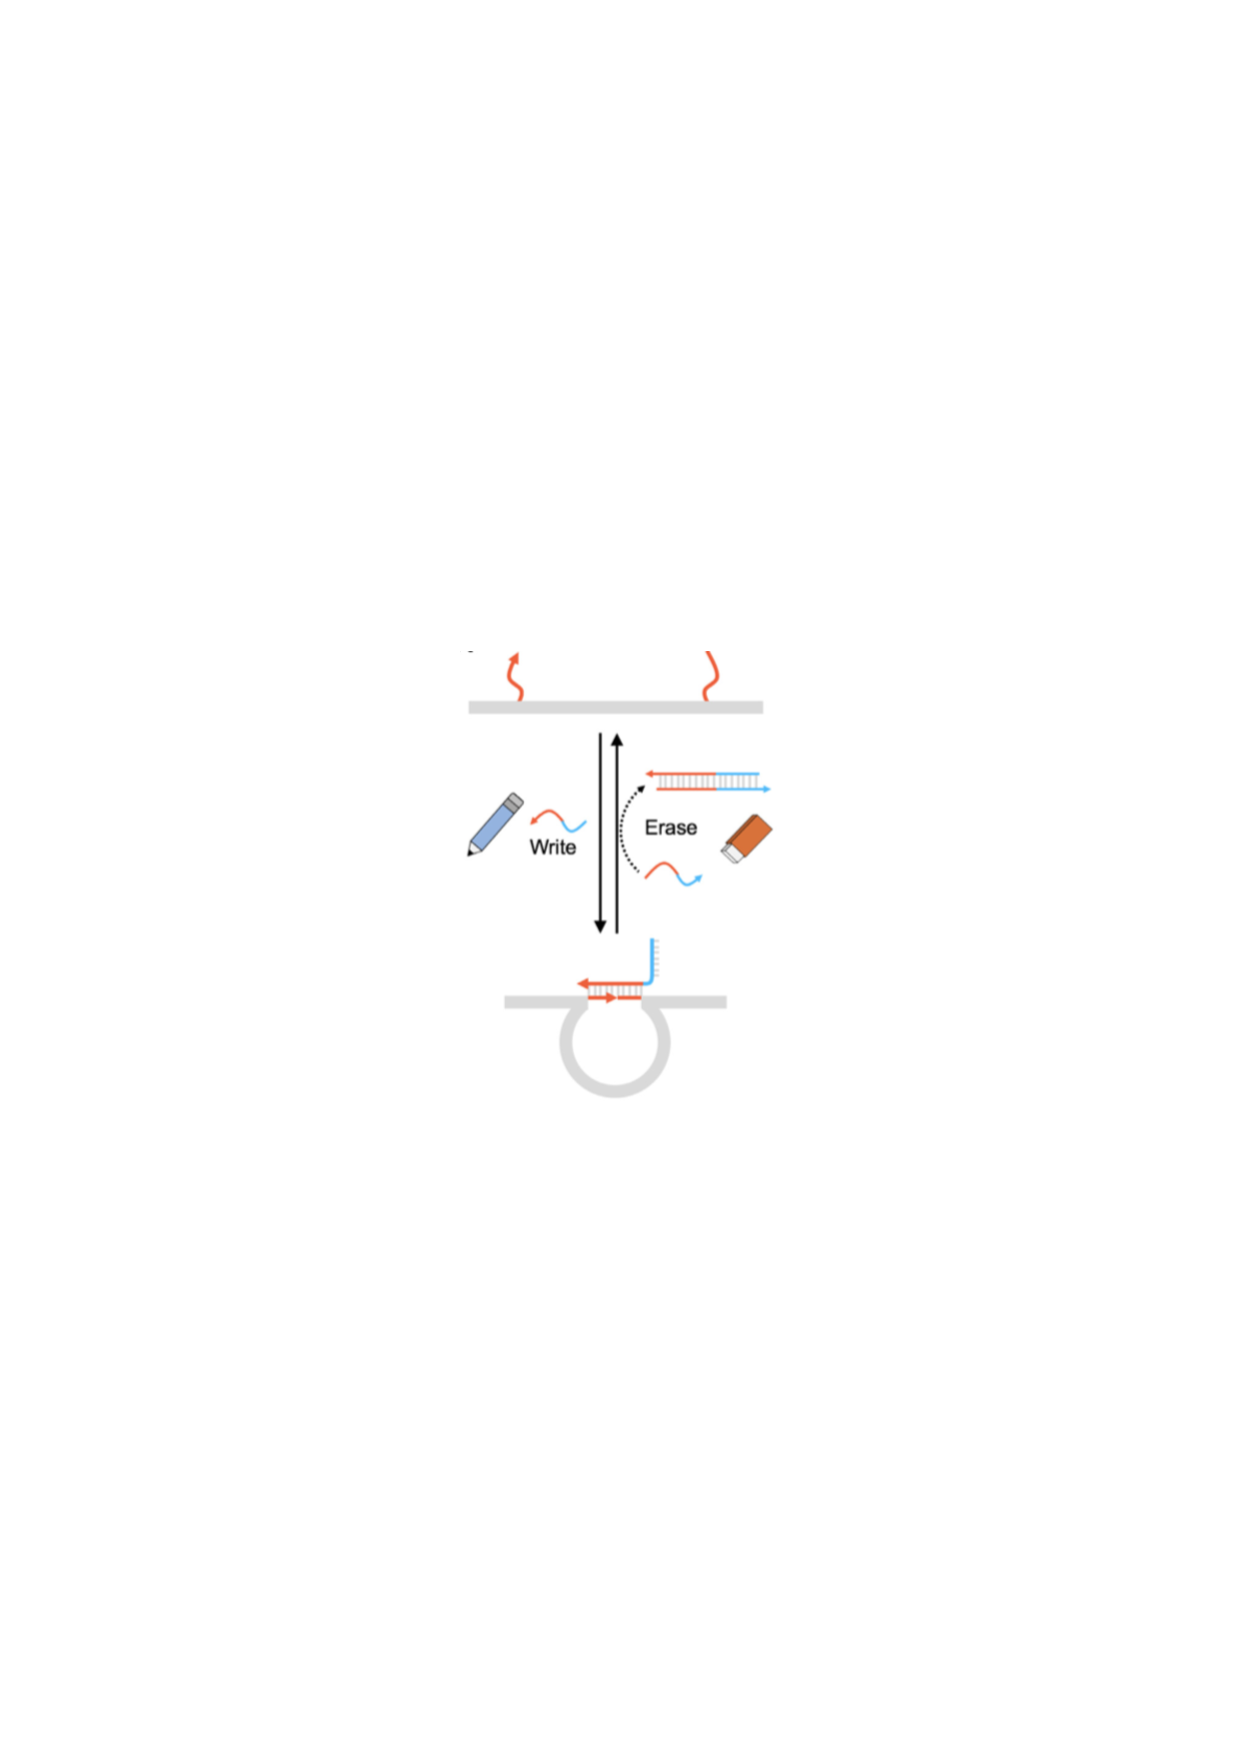
\includegraphics[width=4cm]{reescritura-2.pdf}
\caption{Esquema de escritura y reescritura.}
\label{fig:reescritura2}
\end{center}
\end{figure}

\subsection{Formato de los datos}

Otro problema de representar datos en el ADN es que la tecnología de síntesis actual no permite generar secuencias grandes de nucleótidos (el máximo teórico esta en 200 y el práctico en 120), por lo tanto, los datos deben dividirse en varias cadenas de ADN. Además, otro objetivo de estas memorias es permitir el acceso a los datos mediante acceso aleatorio, es decir, obtener únicamente un dato concreto sin tener que descodificar todas las cadenas de ADN.

Para poder almacenar grandes archivos, \citep{Goldman2013} propusieron una codificación que segmentaba los datos en diferentes cadenas, y almacenaba en unos nucleótidos prefijados, que actúan como segunda cabecera, la información relativa a la localización (o posición) del segmente en el archivo. De esta manera, archivos de gran tamaño pueden descomponerse en pequeños fragmentos y desordenarse, y aún así se puede reconstruir el archivo original.

Para poder extraer la información se utiliza la técnica de amplificación con PCR comentada anteriormente. Generalmente las cabeceras \textit{5’} y \textit{3’} eran comunes entre todas las cadenas de ADN sintetizadas de manera que cuando se quería extraer la información, con un único cebador se podían amplificar todos los datos. Sin embargo, para poder acceder de manera aleatoria a los datos sin necesidad de descodificar todo el ADN, en el \cite{Bornholt2017} se propuso el uso de un sistema de diccionario \textit{clave-valor}. La metodología propuesta mapea la clave de cada fichero a un cebador único de tal manera que, cuando se quería obtener solamente un documento concreto, mediante PCR se amplificaban solo las cadenas con el cebador seleccionado y podía extraerse el documento completo (Figura \ref{fig:dataformat}). Con esta técnica, cada fichero tiene una cabecera única y diferente, y dentro del mismo archivo, todas las cadenas tienen la misma cabecera, pero cambiarán los nucleótidos de posicionamiento.

\begin{figure}[h!]
\begin{center}
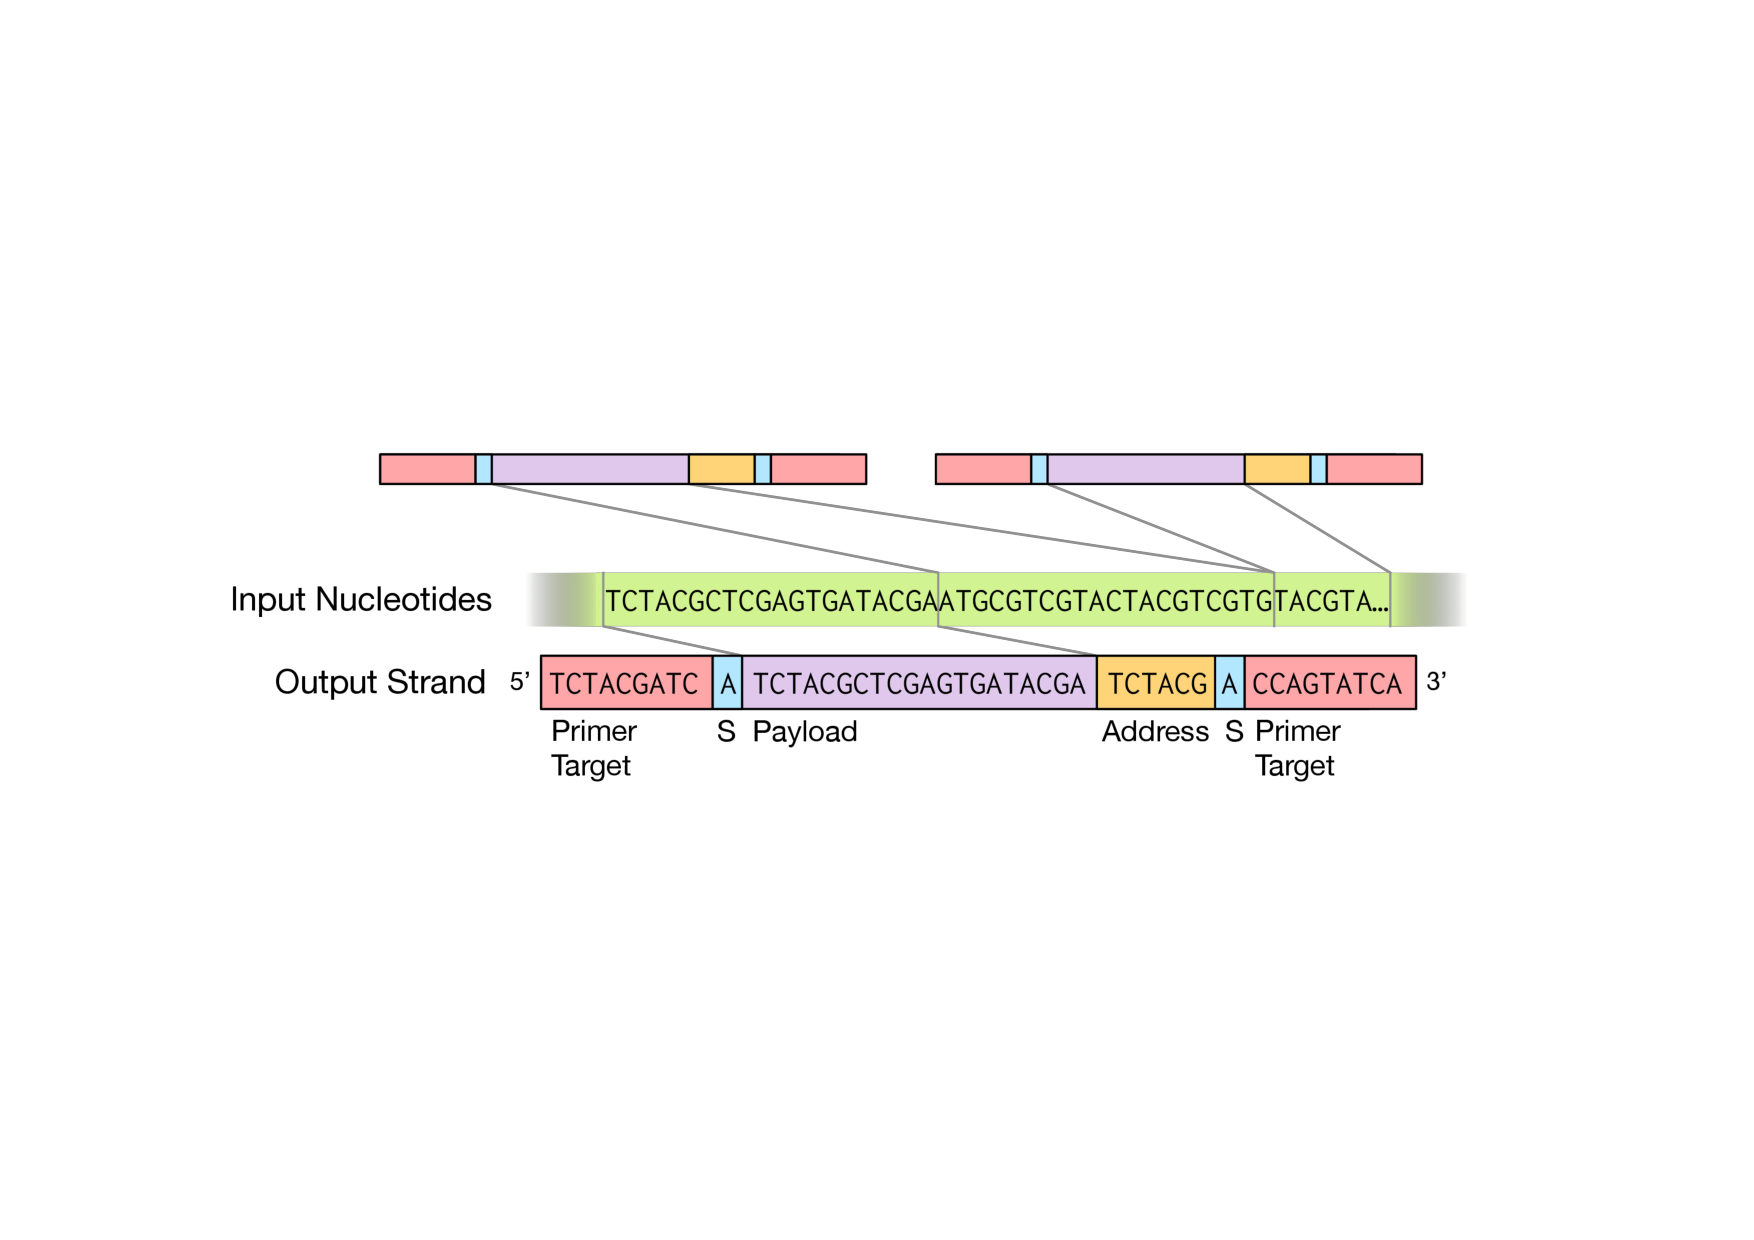
\includegraphics[width=0.82\linewidth]{data-format.pdf}
\caption{Estructura de las cadenas de ADN compuesta por datos, direccionamiento y cabeceras.}
\label{fig:dataformat}
\end{center}
\end{figure}

\subsection{Métodos de codificación}

En las secciones anteriores se ha descrito cómo los datos se pueden dividir en cadenas de ADN. Sin embargo, la codificación implícita que ello conlleva es \textit{naive}: cada bit de datos binarios se codifica en una única cadena de ADN de salida, y por lo tanto no hay robustez o inmunidad ante fallos en la transcripción o síntesis del ADN. Por ello se muy importante un nuevo sistema más fiable. 

En esta sección se van a analizar diferentes propuestas de codificación que obtienen buenos valores para la ratio de confiabilidad-densidad implícito en el diseño. Esto se debe a que, en lo métodos actuales, cuanto mayor es la confiabilidad (mayor redundancia de la información), menor es la densidad de ADN y, por tanto, se pueden almacenar menos datos.


\subsubsection{Codifiación Goldman}

La codificación propuesta por \citep{Goldman2013}, que se muestra en la Figura \ref{fig:goldmancoding}, divide los nucleótidos de ADN de entrada en segmentos disjuntos. Para obtener redundancia, se utiliza una ventana móvil de cuatro segmentos, de forma que las cadenas de ADN estén formadas por cuatro segmentos, y cada segmento aparezca en 4 cadenas. Los autores utilizaron esta codificación para recuperar con éxito un mensaje de 739 kB.

\begin{figure}[h!]
\begin{center}
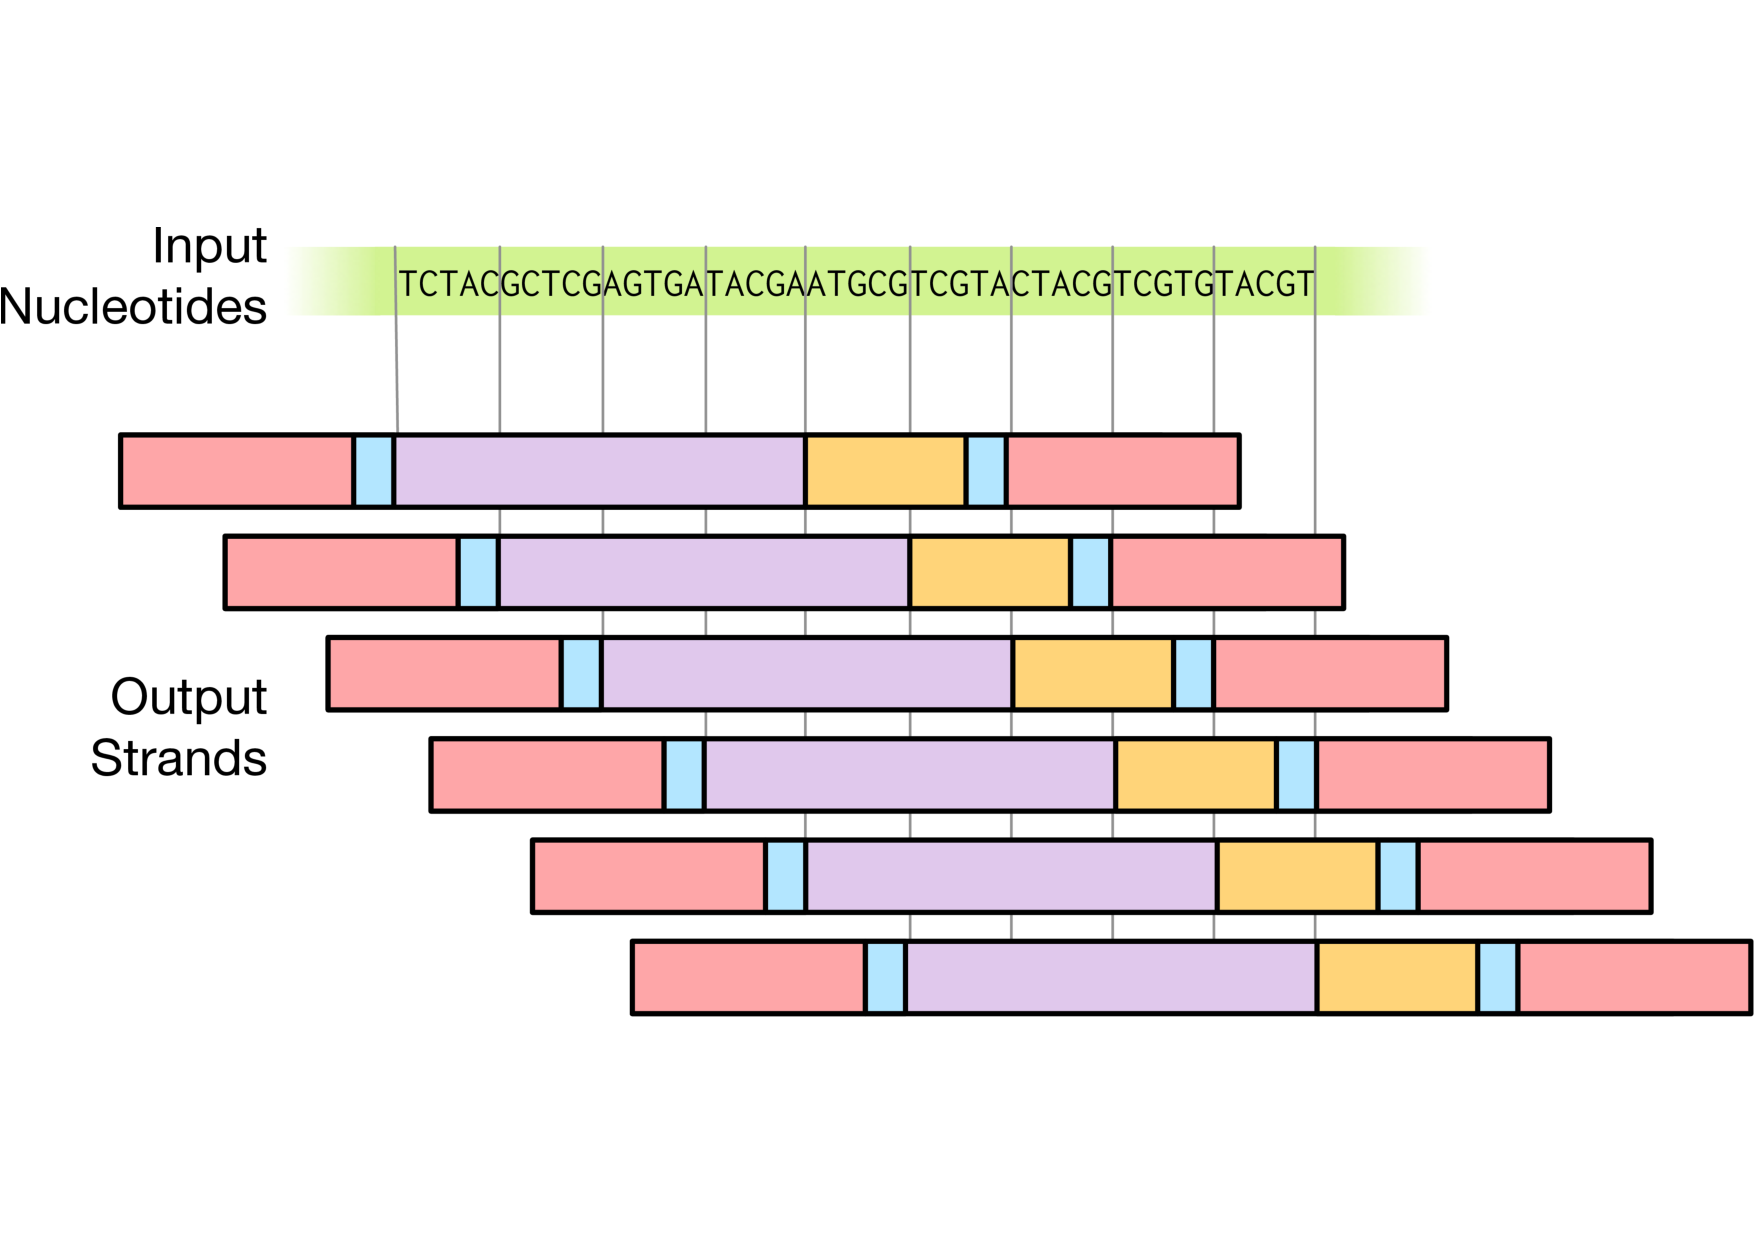
\includegraphics[width=0.75\linewidth]{goldman-coding.pdf}
\caption{Método de codificación de Goldman. Separación de la cadena de datos en segmentos y utilizando una ventana de cuatro partes, se transcriben a los nucleótidos del ADN.}
\label{fig:goldmancoding}
\end{center}
\end{figure}

Este método ha sido extensamente utilizado en la literatura y esta considerado uno de los más robustos. Además, da la posibilidad de ajustar el nivel de redundancia (y por tanto el nivel de densidad), ya que si en vez de introducir cuatro segmentos por cada cadena, se utilizasen segmentos más grandes y se introdujesen solo tres o dos, el nivel de redundancia sería menor. En caso de coger segmentos mayores, el nivel de redundancia sería mayor.

\subsubsection{Codificación XOR}

La codificación Goldman proporciona una alta confiabilidad, pero a su vez genera una gran sobrecarga: cada bloque en la cadena de entrada se repite cuatro veces. Por este motivo, aunque el método de Goldman se sigue utilizando ampliamente, se han propuesto nuevos métodos tales como el de \cite{Bornholt2017} llamado codificación XOR (también llamada OR exclusiva).

\begin{figure}[h!]
\begin{center}
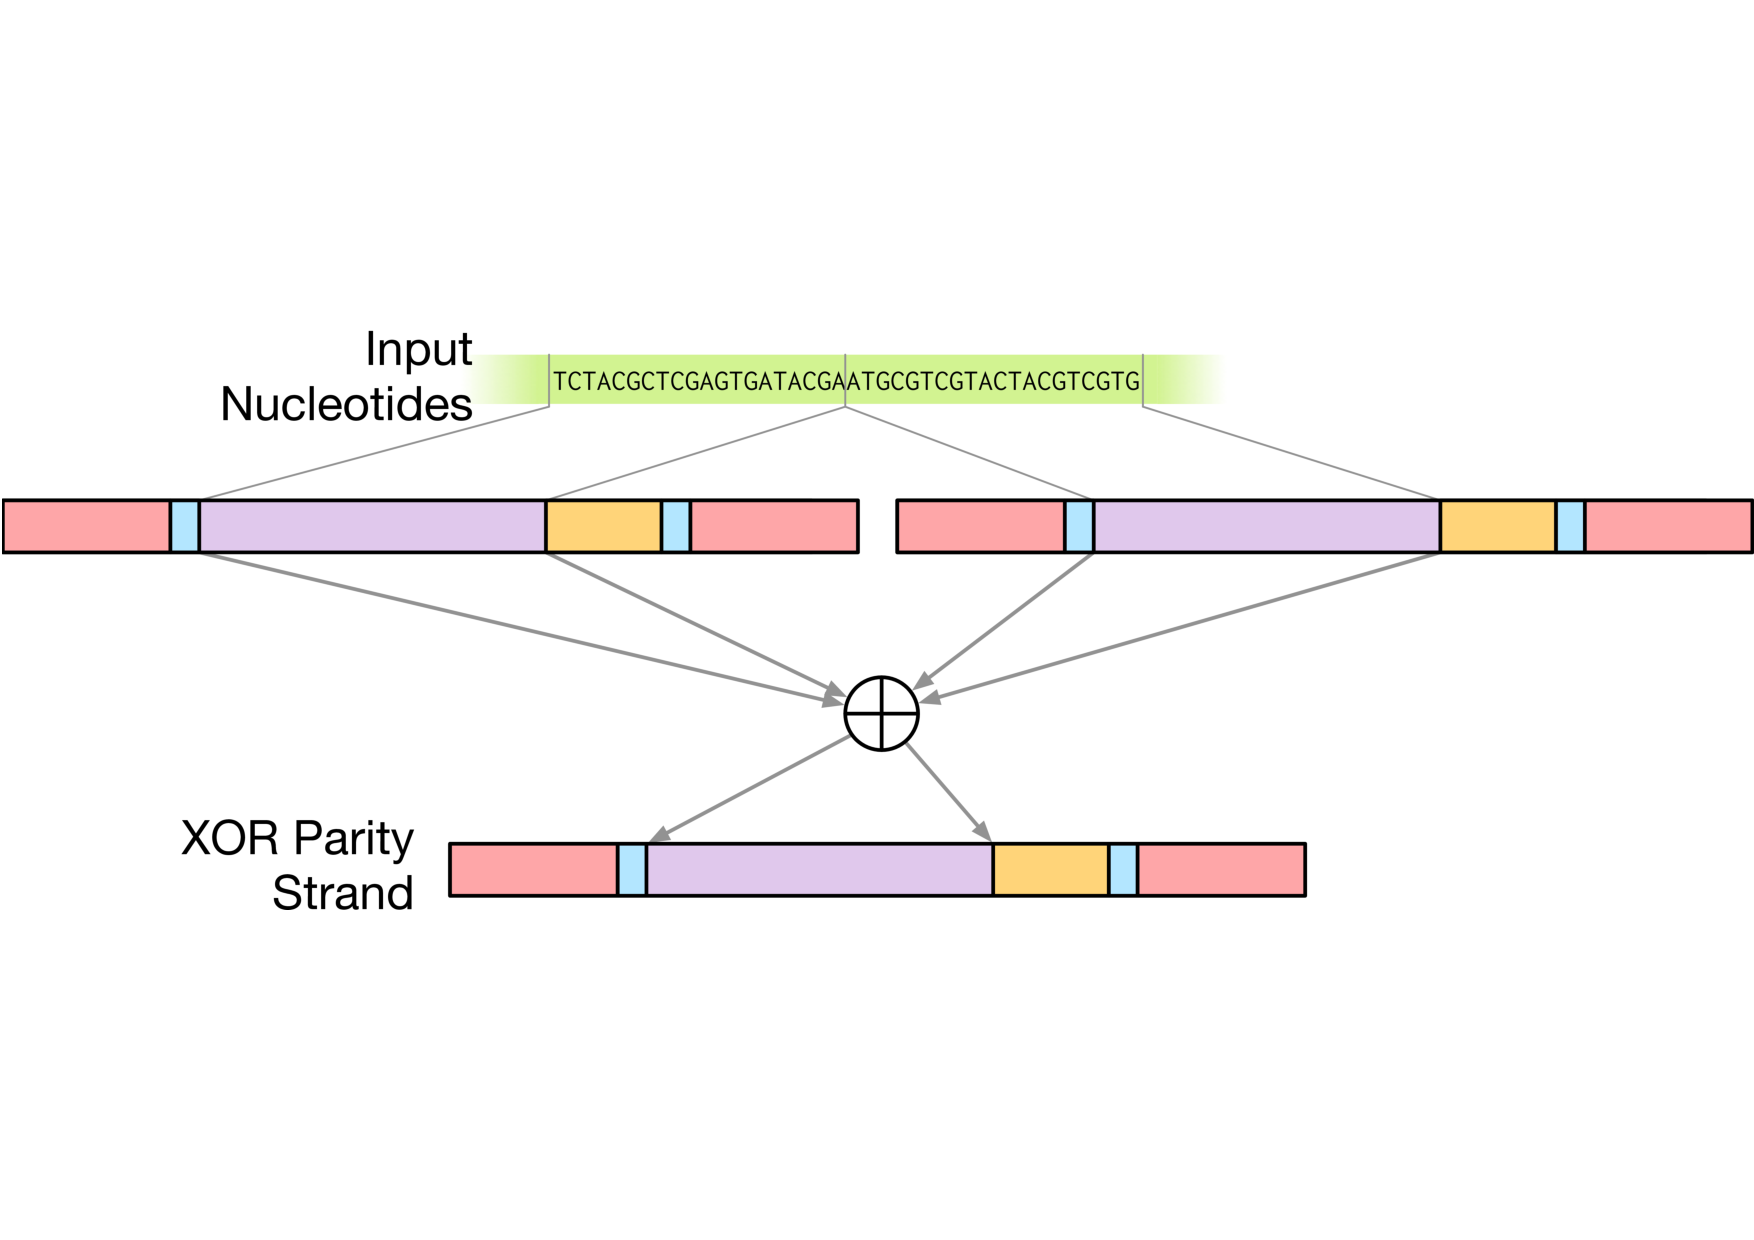
\includegraphics[width=0.75\linewidth]{xor-coding.pdf}
\caption{Método de codificación XOR. Utilizando el operador OR exclusivo entre dos cadenas de ADN obtenemos una tercera que nos sirve para reconstruir las otras dos en caso de que una de ellas tuviera fallos.}
\label{fig:xorcoding}
\end{center}
\end{figure}

Este método tal y como se muestra en la Figura \ref{fig:xorcoding}, proporciona redundancia mediante el uso de la operación OR exclusiva. La idea principal del método consiste en coger la carga útil de dos cadenas de ADN y utilizando el operador XOR entre ellas, \(A \bigotimes B\), obtener una tercera cadena que sirva de complementaria a aquellas. Además, para identificar que esta nueva cadena generada es la XOR de A y B, se almacenará esta información en los nucleótidos de direccionamiento de la cadena (sección naranja de la cadena de ADN). Con esta arquitectura, teniendo únicamente dos de las tres cadenas se puede recuperar la tercera (es para el caso de haberla perdido o fallos en la transcripción o síntesis).

Tal y como se describe en el artículo, la fiabilidad de esta codificación es similar a la de Goldman. Sin embargo, la densidad teórica de la codificación XOR es mucho menor que la de Goldman, dado que en esta cada nucleótido se repite cuatro veces y, sin embargo, en la XOR cada nucleótido se repite 1.5 veces.

Este tipo de codificación puede modificarse de igual manera que el propuesto por Goldman para aumentar la densidad del ADN reduciendo la fiabilidad del sistema. Por ejemplo, si en vez de dos cadenas utilizásemos 4, aplicaríamos el operador OR exclusivo sobre los 4 y generaríamos una quinta cadena que serviría para reconstruir la faltante en caso de que algunas de las 4 sufriera fallos. De esta manera, se reduce la robustez del sistema, pero se consigue una mayor densidad de ADN.

\subsection{Evolución histórica}
En las últimas dos décadas, tal y como se muestra en la Figura \ref{fig:ordendescubrimientos} \citep{DeSilva2016}, se ha investigado mucho en este campo. Esto es debido al gran potencial de la computación con ADN y a la gran expectación que ha generado. En esta sección se van a mencionar brevemente algunos de los proyectos mas relevantes en el ámbito del almacenamiento de información en ADN.

\begin{figure}[h!]
\begin{center}
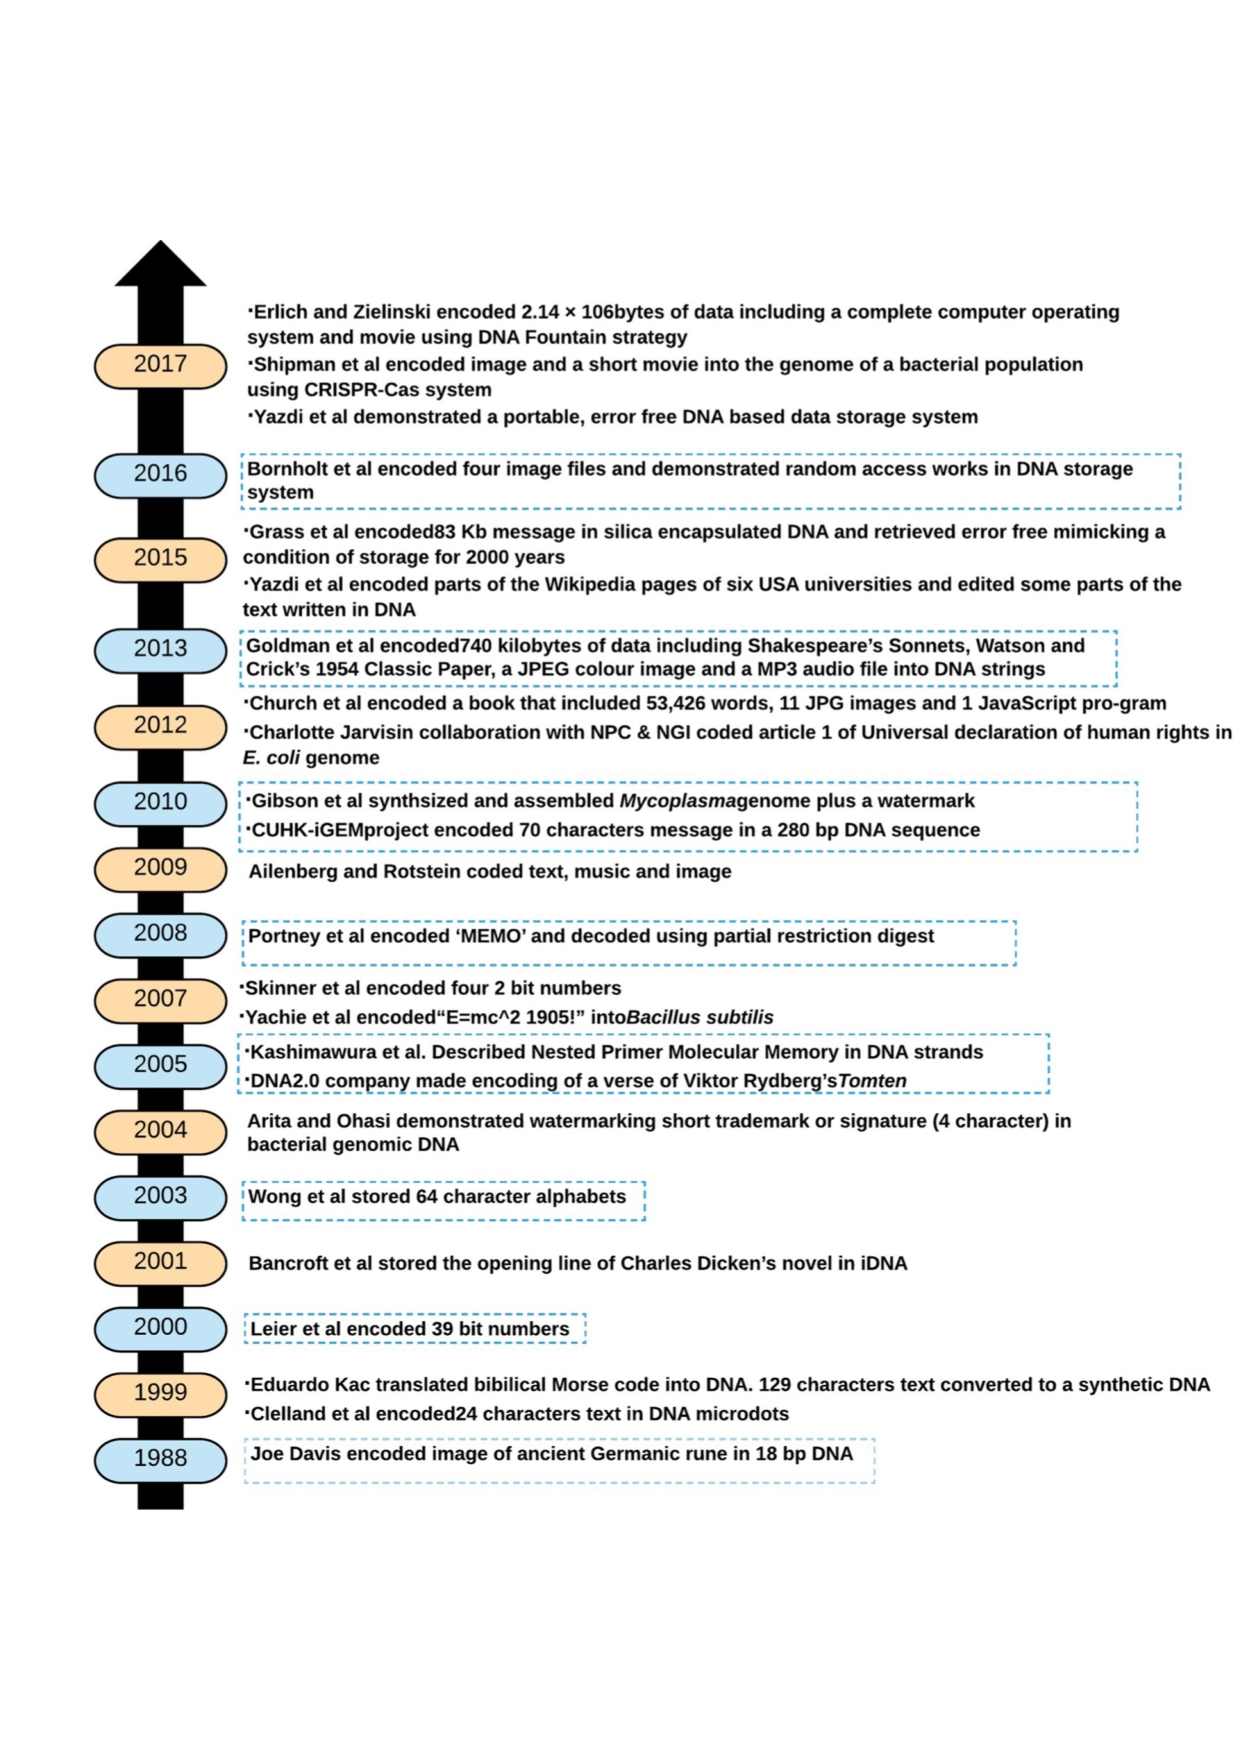
\includegraphics[width=0.75\linewidth]{orden-descubrimientos.pdf}
\caption{Investigaciones de las ultimas dos décadas sobre almacenamiento en ADN.}
\label{fig:ordendescubrimientos}
\end{center}
\end{figure}

Para no entrar en una descripción detallada, se va a ampliar a continuación dos de los proyectos pioneros en el almacenamiento de información utilizando memorias de ADN:

\subsubsection{Proyecto Microvenus}

Este proyecto fue iniciado por \citep{JoeDavis1996} para almacenar una imagen en ADN. La codificación se basó en el tamaño molecular de las bases, \(C \rightarrow 1, T \rightarrow 2, A \rightarrow 3\) y \(G \rightarrow 4\). Con este ajuste de referencia, la codificación se basó en traducir los bits a nucleótidos en función del número de veces que aparecieran repetidos el \textit{0} o el \textit{1}. Así, si aparecía un \textit{1} o un \textit{0} se pondría una \textit{C}, si aparecían dos \textit{1} o dos \textit{0} se pondría una \textit{T} y así sucesivamente hasta 4. Con este mapeo se obtenían, por ejemplo, las siguientes conversiones: \textit{100101 = CTCCT} y \textit{10101 = CCCCC}. 

El principal inconveniente venía en la decodificación, donde una C podría decodificarse como \textit{1} o \textit{0}, porque solo se tomó en cuenta el número de bits repetidos en el momento de la codificación. Por ejemplo, el \textit{CTCCT} se podría descodificar como \textit{011010} o \textit{100101}. 

\subsubsection{Proyecto Génesis}

 Pocos años después, \citep{EK1999}, partiendo de un fragmento del libro \textit{ “Génesis”}, lo transformó a Morse y diseño un sistema de codificación de Morse a nucleótidos. Esencialmente el sistema codificaba los guiones y los puntos como \textit{T} y \textit{C}, respectivamente y los espacios entre letras y entre palabras con \textit{A} y \textit{G}, respectivamente.
 
Los genes sintéticos se fusionaron en bacterias y, en presencia de una luz ultravioleta, se produjeron mutaciones en las bacterias que provocaron fallos en los genes visibles en la descodificación.\\

Estos dos métodos sentaron las bases para la codificación en el ADN, pero no han continuado siendo utilizados.

\section{Conclusiones}

La computación con ADN ha tenido un gran auge en los últimos años debido a la gran expectación que ha generado. Este se debe al alto potencial que tiene esta tecnología y la inmensa cantidad de posibilidades que brinda a los investigadores. Por ello, han surgido gran cantidad de ramas de investigación, entre ellas, la creación de memorias basadas en ADN.

Tal y como se ha mostrado en este documento, ha habido un gran progreso y se han logrado grandes avances e hitos. En mi opinión es una vía de trabajo que tiene futuro y que posiblemente algún día se llegue a productivizar y a utilizar a gran escala.
Sin embarga, en mi opinión, hoy en día es una tecnología aún por madurar y con mucho que demostrar. Los trabajos que hay hasta el momento han sido en su mayoría pruebas de concepto y demostraciones para sentar las bases de lo que será en unos años una importante línea de trabajo.

Uno de los grandes inconvenientes que tiene hoy en día esta tecnología es la escalabilidad. Por ejemplo, en las propuestas para el método de sobreescritura utilizando \textit{hairpins} o los sistemas de direccionamiento para distinguir entre bloques dentro de un mismo documento no son escalables. En el caso de los \textit{hairpins} se requieren muchos nucleótidos para formar un sistema de más de 10 bits y, además, para cada bit necesitamos una cadena de ADN diferente, o solapar más de uno en una misma cadena (lo cual volvería a agravar el problema de utilizar demasiados nucleótidos por bit). En el caso del direccionamiento, si por ejemplo se reservan 5 nucleótidos para la identificación del bloque, solo se podrían codificar 25 bloques, lo cual puede ser insuficiente en ciertas situaciones. Para este último caso, en concreto, se necesita que mejore la capacidad de nucleótidos por cadena de ADN actual, ya que los 200 teóricos (120 en la práctica) no son suficientes para este tipo de problemas.

Otro problema es el de los fallos en la transcripción o síntesis, así como las mutaciones aleatorias que sufren las células. Los sistemas de redundancia que se han comentado en el articulo y que se están utilizando en la literatura, mitigan este tipo de problemas. Sin embargo, siguen si proporcionar una fiabilidad como la de los sistemas tradicionales de almacenamiento y, además, reducen la densidad del ADN (al haber más redundancia, hay menos información en la misma cantidad de ADN). Por lo tanto, aunque se están consiguiendo buenos avances en este aspecto, considero que es una vía a tener en cuenta y mejorar.

A pesar de esto, el decremento en los costes de síntesis de ADN, el gran potencial de la tecnología y que el ADN es consustancial al ser humano, hacen su estudio ineludible y convierten a las memorias de ADN en un tema muy interesante para los investigadores y que tendrá grandes avances en los próximos años.



\newpage

%%\bibliography{biblio1} 
%%\bibliographystyle{plainnat}
\printbibliography

\end{document}
